\subsection{Test de isoterma en función de las condiciones de borde}

La temperatura interna y externa aumentan a la misma velocidad. La isoterma buscada en todos los
casos es de $1500 ^{\circ}C$.

\begin{figure}[H]{}
\centering
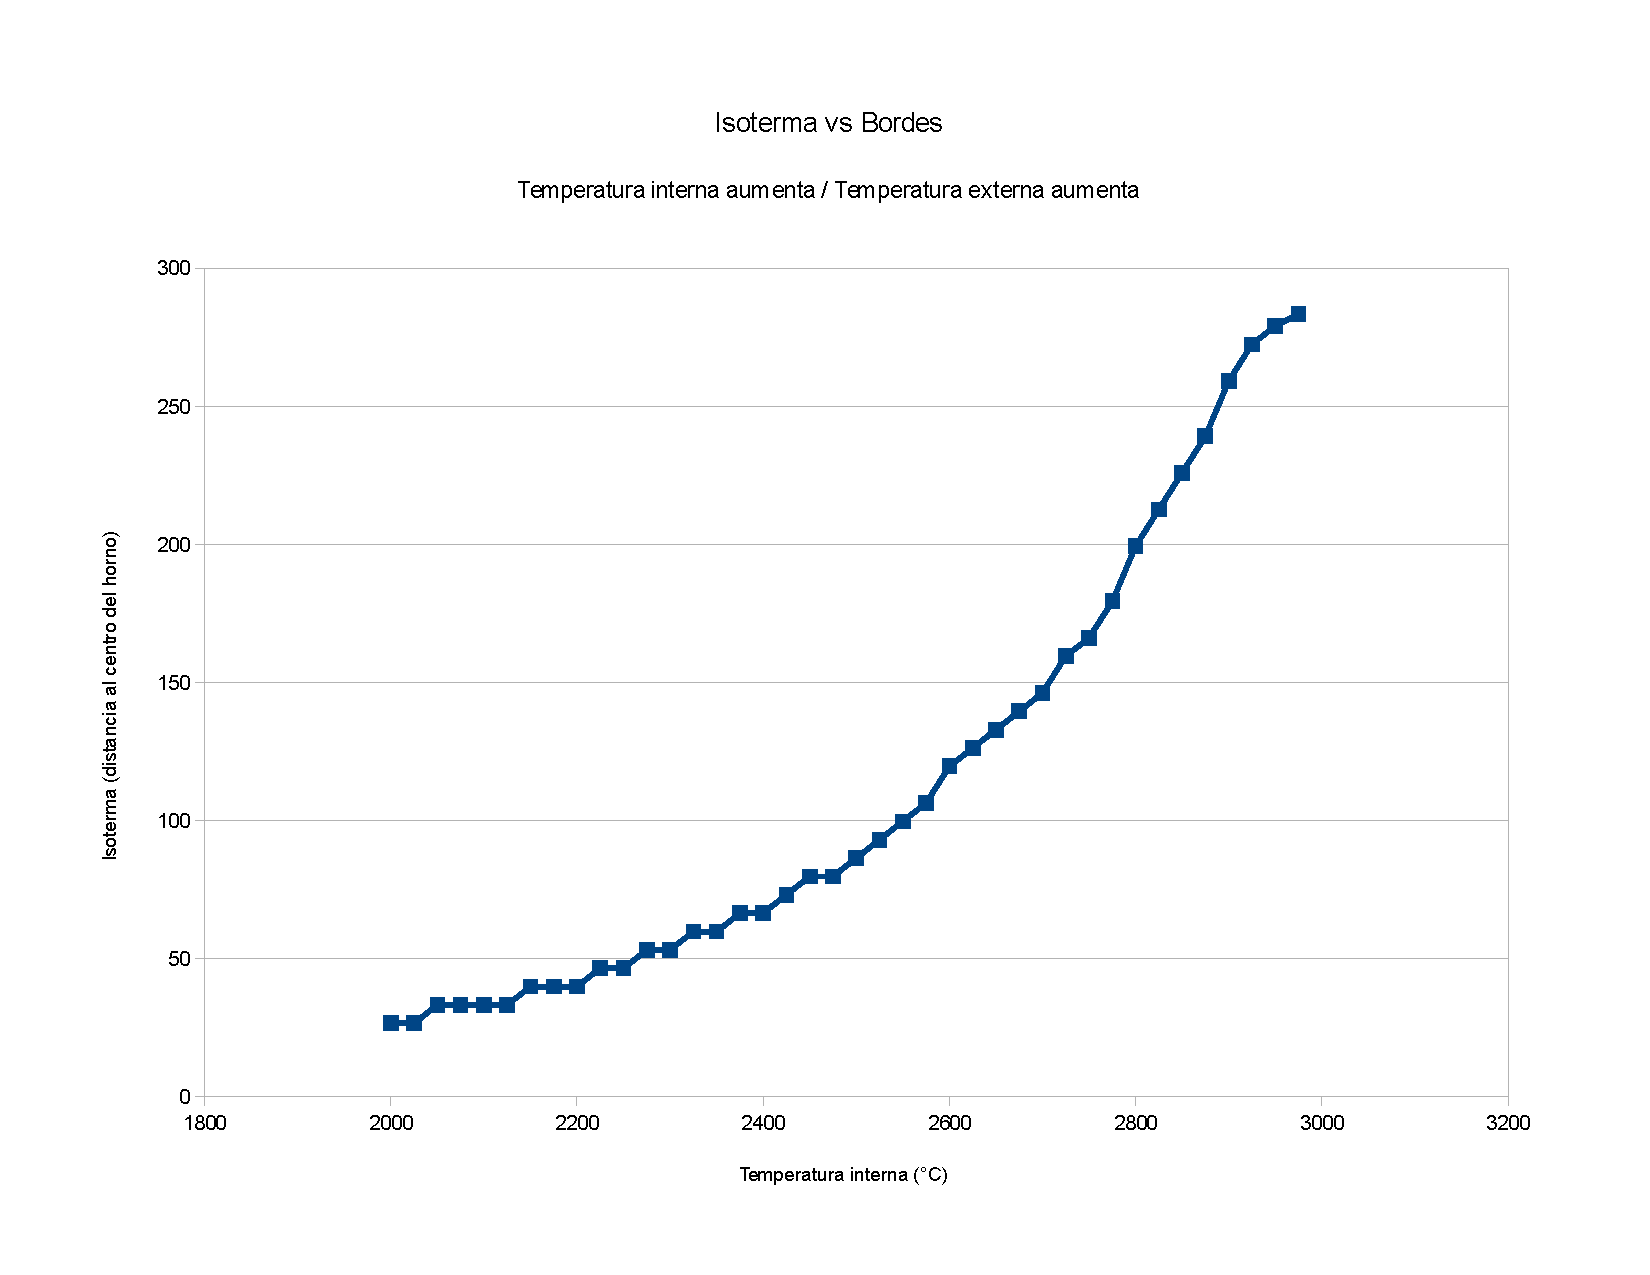
\includegraphics[scale=0.5]{graphs/isotermaVsBordesExternaAumenta.pdf}
\caption{La temperatura externa e interna a aumentan con la misma proporción. La temperatura externa empieza en 0 $^{\circ}C$}
\label{isotermaVsBordesExternaAumenta}
\end{figure}

\begin{figure}[H]{}
\centering
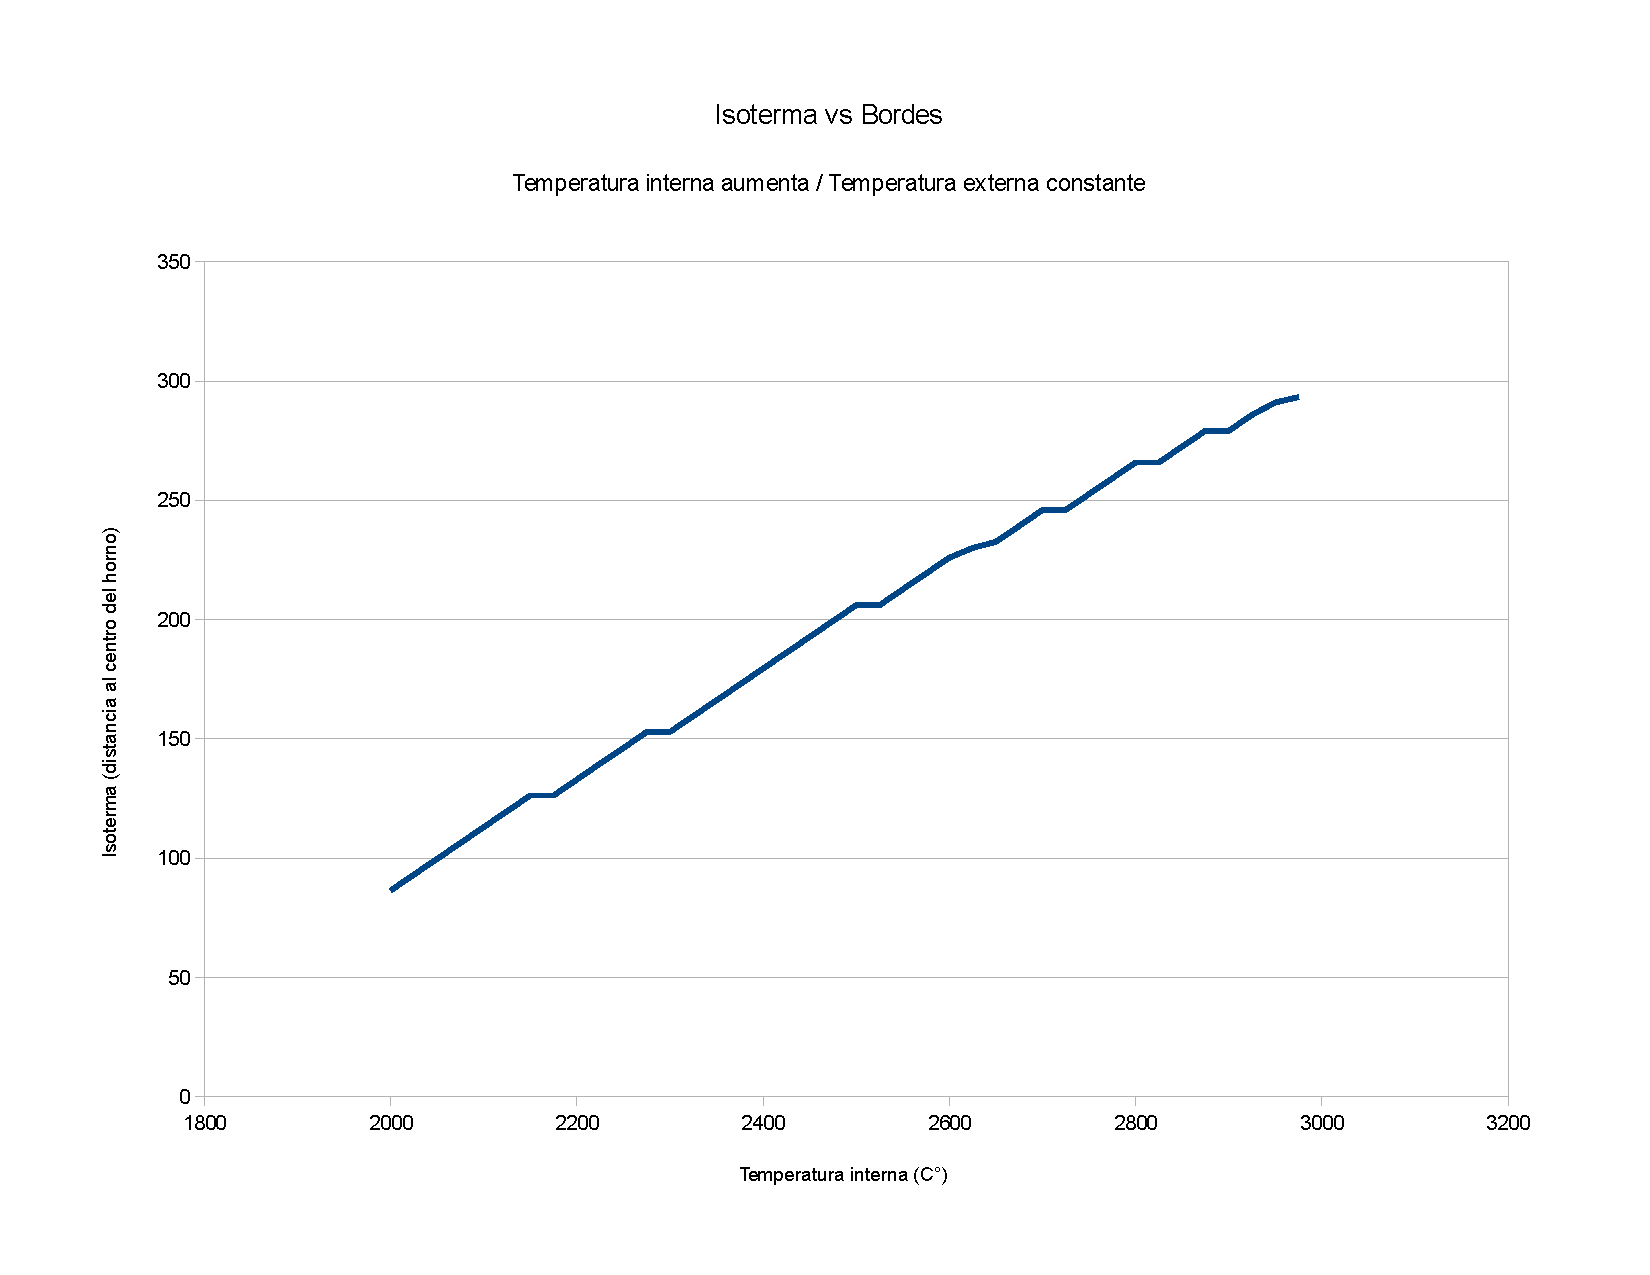
\includegraphics[scale=0.5]{graphs/isotermaVsBordesExternaConstante.pdf}
\caption{La temperatura externa se mantiene constante a 1000 $^{\circ} C$}
\label{isotermaVsBordesExternaConstante}
\end{figure}

La temperatura externa desciende a un $40\%$ la velocidad a la que aumenta la temperatura interna.

\begin{figure}[H]{}
\centering
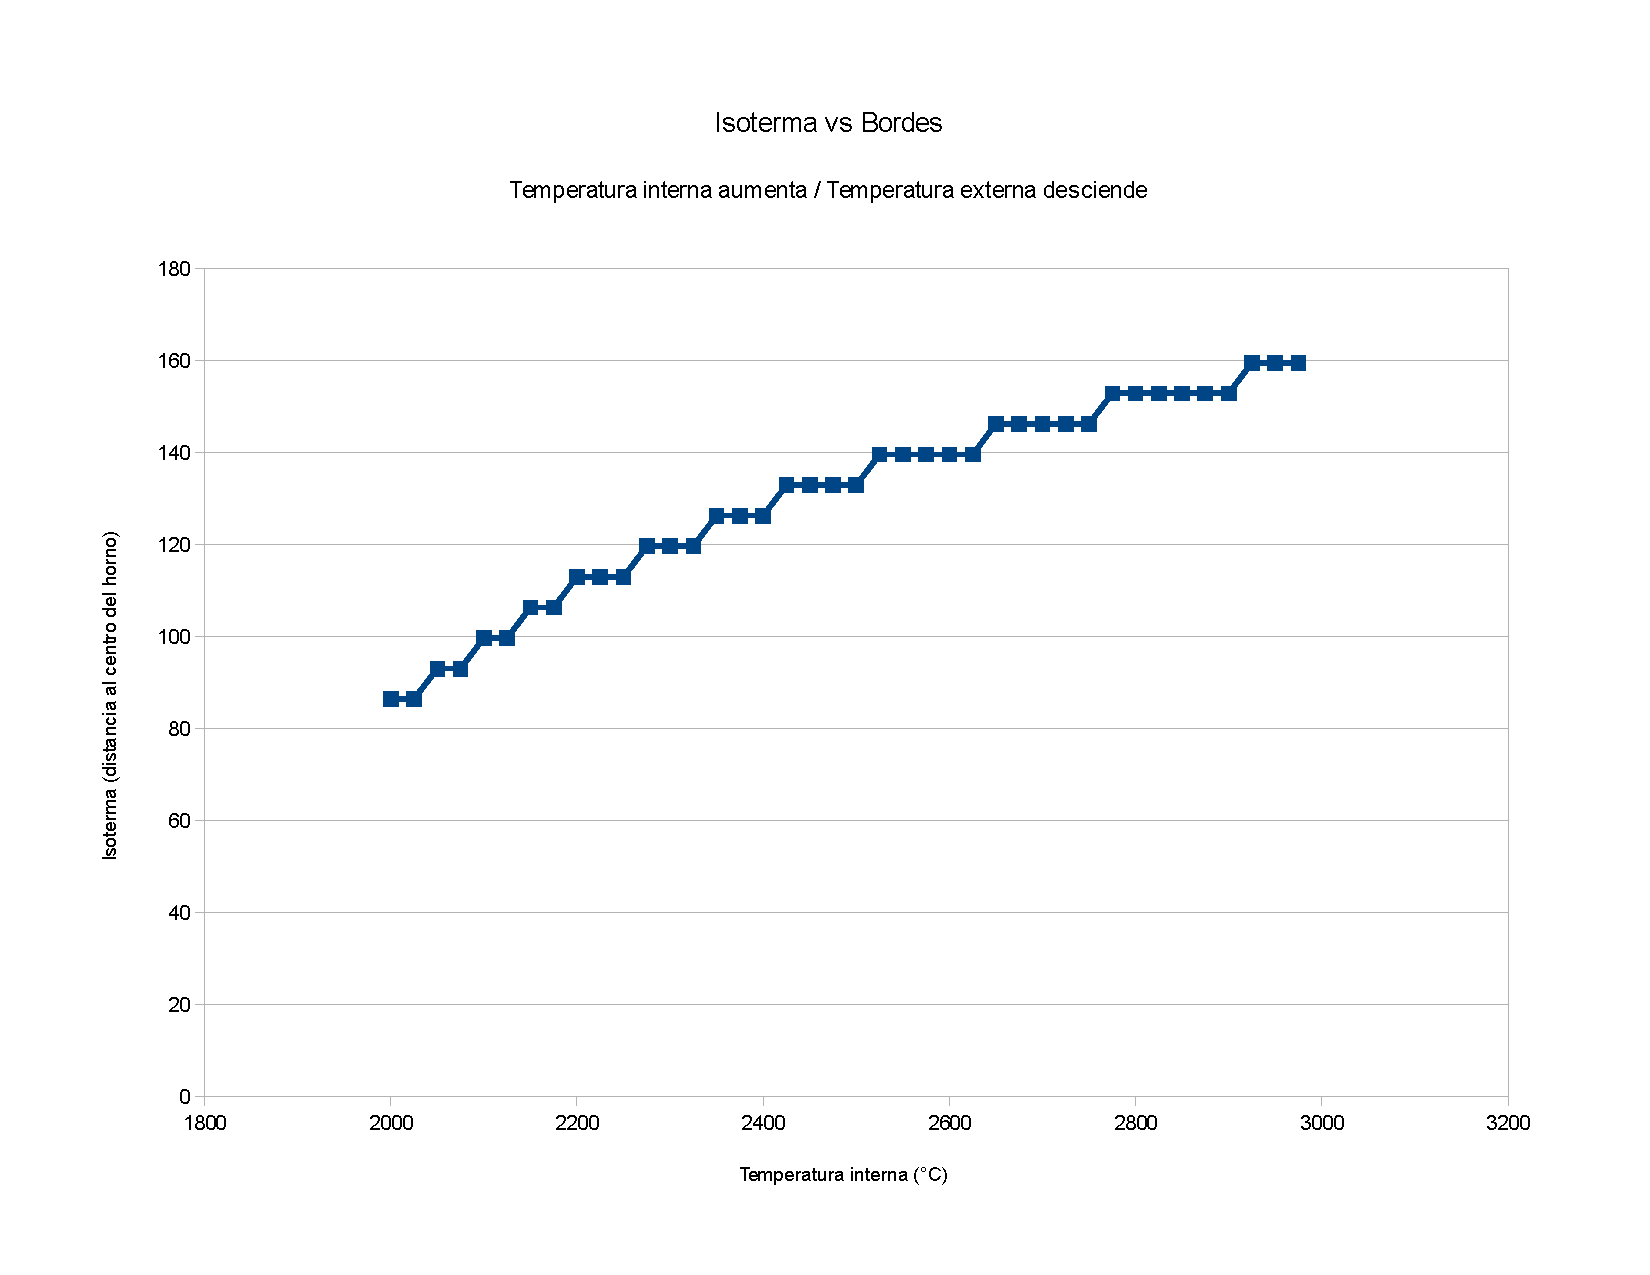
\includegraphics[scale=0.5]{graphs/isotermaVsBordesExternaDesciende.pdf}
\caption{La temperatura externa desciende más lento que lo que aumenta la interna.}
\label{isotermaVsBordesExternaDesciende}
\end{figure}
